\section{Synthesis: which engine, and when}
\label{discussion:synthesis-which-engine-when}

% RQ3 + decision synthesis. Reads Section~\ref{results:consistency-of-winners} and pulls
% Sections 7.1--7.2 together. This section carries goal 2: implementation/complexity cost
% weighed against usage cost.
%
% Points to cover:
% - No single winner across dimensions: PostGIS leads single-machine time, Sedona leads the
%   distributed join from the medium tier, the cost winner is mixed
%   (Figure~\ref{fig:winners-matrix}, Table~\ref{tab:geomean-normalized-performance}). Argue
%   "best engine" is ill-posed without fixing workload, tier, and outcome dimension.
% - Outcome inversions: time and cost orderings cross
%   (Figure~\ref{fig:outcome-parallel-coordinates}, Figure~\ref{fig:rank-portability}); a
%   near-flat rank line can hide more than two orders of magnitude in absolute terms. Tie the
%   time/cost split to per-resource metering and, for Sedona, node-hour + provisioning billing
%   (Section 2.1.4, 2.4.5)
%   \parencite{mell2011_nist_definition_of_cloud_computing,databricks2024_cost_optimization_best_practices}.
% - Rank inversions are tier-dependent only for the join
%   (Figure~\ref{fig:ranking-stability}); the single-machine patterns are rank-stable across
%   tiers. Tie to range-query vs join exercising the lifecycle differently
%   \parencite{yu2019_geospark_perspective_beyond}.
% - DECISION FRAME (goal 2): map findings onto complexity/implementation cost vs usage cost.
%   Tuned single-node PostGIS for single-machine analytical queries; distributed Sedona once
%   data exceeds single-node memory; DuckDB's value is operational (flat transfer, low cloud
%   cost) rather than latency. Mark tied regions "either"; mark untested boundaries as extrapolation.
%
% FIGURE 1 (Lucidchart, to produce): "which engine when" decision quadrant, built from the
%   measured winners, crossover points, and significance results; tied regions read "either";
%   boundaries beyond the tested tiers marked as extrapolations. Uncomment when the file exists.
% \begin{figure}[H]
%     \centering
%     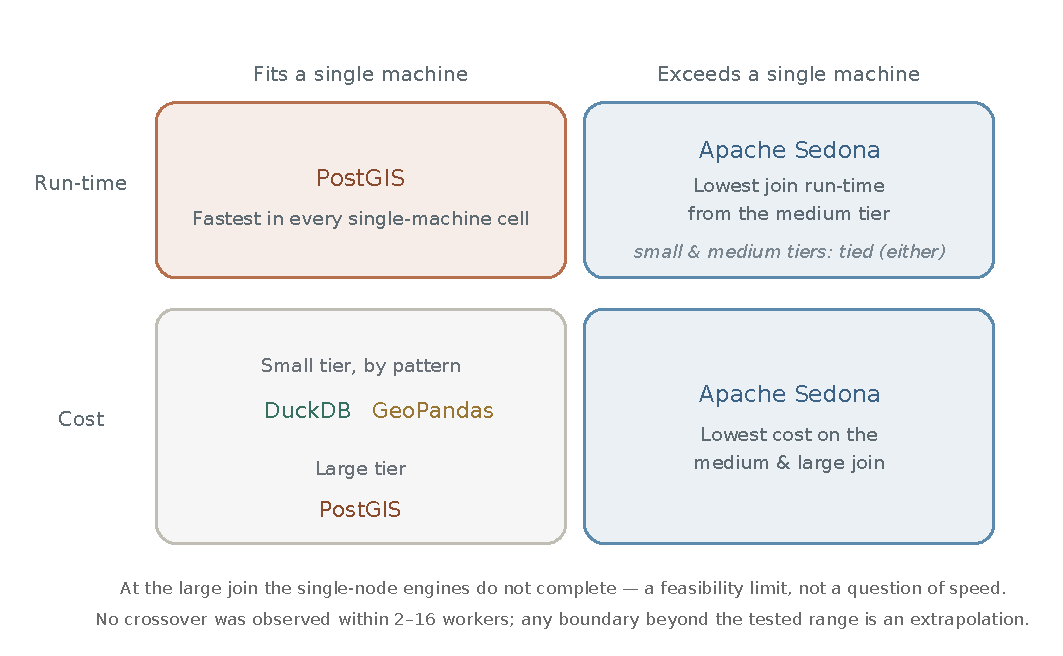
\includegraphics[width=0.85\textwidth]{Chapters/07-discussion/sub-chapters/figures/07-decision-quadrant.pdf}
%     \caption[Decision quadrant: which engine when]{TODO caption.}
%     \label{fig:discussion-decision-quadrant}
% \end{figure}
%
% FIGURE 2 (Lucidchart, to produce): complexity / implementation cost vs usage (operational)
%   cost map, positioning each configuration on the two axes that frame the decision (goal 2).
% \begin{figure}[H]
%     \centering
%     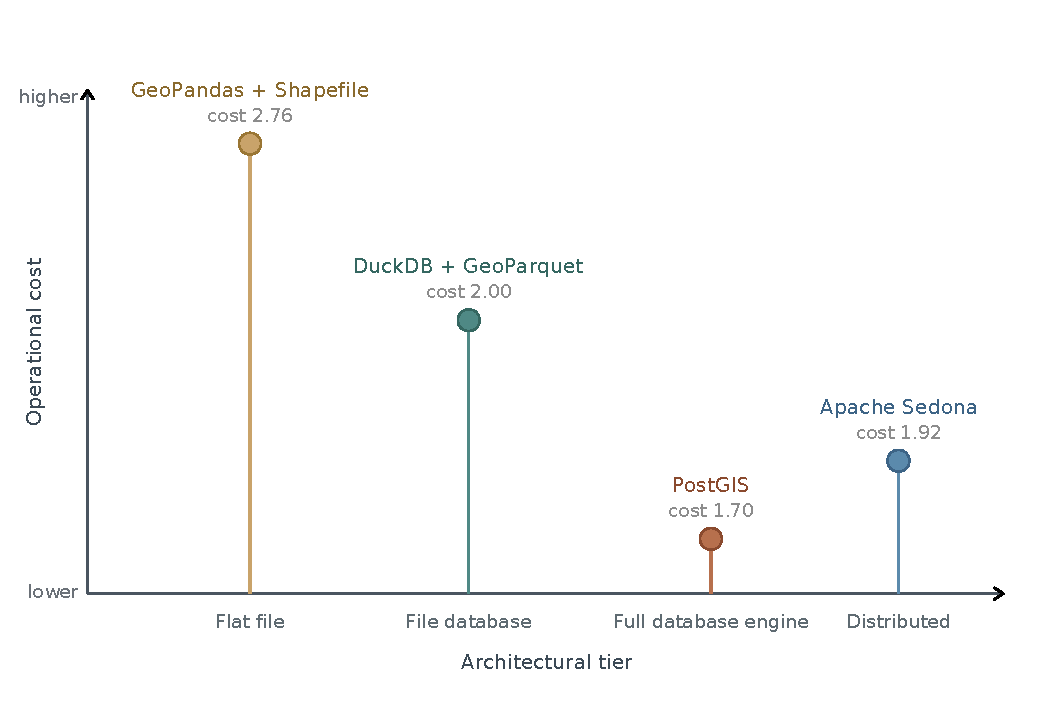
\includegraphics[width=0.85\textwidth]{Chapters/07-discussion/sub-chapters/figures/07-complexity-vs-cost.pdf}
%     \caption[Complexity versus operational cost]{TODO caption.}
%     \label{fig:discussion-complexity-vs-cost}
% \end{figure}